\documentclass[12pt,a4paper]{article}

% Pacchetti per la lingua e i font
\usepackage[utf8]{inputenc}
\usepackage[italian]{babel}
\usepackage[T1]{fontenc}

% Pacchetti matematici fondamentali
\usepackage{amsmath}
\usepackage{amsfonts}
\usepackage{amssymb}

% Pacchetto per la notazione fisica (Bra-Ket)
\usepackage{physics} 

% Per margini più simili all'immagine
\usepackage[margin=1in]{geometry}

% Per includere immagini
\usepackage{graphicx}

% Per tabelle pulite
\usepackage{booktabs}

% Per numeri e incertezze
\usepackage{siunitx} 

% Per posizionare le figure con [H] (qui e non flottante)
\usepackage{float}

% Per subfigure
\usepackage{subcaption}

% Distanzia la didascalia dalla tabella
\usepackage[skip=10pt]{caption}


\title{\textbf{Studio dell'oscillatore armonico quantistico nel formalismo del path integral tramite MCMC}}
\author{Tommaso Serra}
\date{\today}

\begin{document}
\maketitle

\section{Introduzione}
In questa relazione viene presentato un semplice studio dell'oscillatore armonico 
quantistico tramite simulazioni Monte Carlo a catena di Markov (MCMC), 
sfruttando la formulazione con l'integrale sui cammini. Viene ricostruita la 
distribuzione di probabilità dello stato fondamentale, vengono stimate le medie 
termiche di alcune osservabili fisiche rilevanti e i primi gap energetici facendo 
uso di opportuni operatori interpolanti e dei loro correlatori connessi.

\subsection{Richiami oscillatore armonico}
L'Hamiltoniana dell'oscillatore armonico è data da:
\begin{equation}
    H = \hat{T} + \hat{V} = -\frac{\hbar^2}{2m} \frac{d^2}{dx^2} + \frac{1}{2}m\omega^2x^2
\end{equation}
i cui autostati in rappresentazione della posizione sono:
\begin{equation}
    \psi_n(x) = \frac{1}{\sqrt{2^n n!}} \left( \frac{m\omega}{\pi\hbar} \right)^{1/4} e^{-\frac{m\omega x^2}{2\hbar}} H_n\left( \sqrt{\frac{m\omega}{\hbar}} x \right)
\end{equation}
dove $H_n$ sono i polinomi di Hermite. I rispettivi autovalori dell'energia sono:
\begin{equation}
    E_n = \hbar\omega \left( n + \frac{1}{2} \right)
\end{equation}

\subsection{Richiami di statistica quantistica e path integral Euclideo}
La funzione di partizione di un sistema quantistico si calcola come:
\begin{equation}
    Z = \text{Tr}(e^{-\beta H})
\end{equation}
Possiamo esprimere la traccia nella base delle posizioni, ottenendo:
\begin{equation}
    Z = \int dx \bra{x} e^{-\beta H} \ket{x}
\end{equation}
Possiamo applicare la procedura del path integral analogamente al caso della propagazione in tempo reale
sfruttando la sostituzione $t \to -i\tau = -i\beta$ passando al tempo immaginario tramite la rotazione di WIck
(l'unica differenza risiede nella necessità di fissare le condizioni al contorno periodiche).
la funzione di partizione in questa formulazione al limite del continuo diventa ($\hbar=1$):
\begin{equation}
    Z \propto \int_{x(0)=x(\beta)} \mathcal{D}x(\tau) e^{-S_E[x(\tau)]}
\end{equation}
dove $S_E$ è l'azione Euclidea data da:
\begin{equation}
    S_E[x(\tau)] = \int_0^\beta d\tau' \left[ \frac{1}{2} m \left( \frac{dx}{d\tau'} \right)^2 + V(x(\tau')) \right]
\end{equation}
A questo punto introduciamo la media termodinamica di un operatore $O$:
\begin{equation}
    \langle O \rangle = \sum_{n} P_{n} O_{n}
\end{equation}
Dove:

\begin{equation*}
    P_{n} = \frac{e^{-\beta E_n}}{Z} \quad\quad\quad O_{n} = \bra{n} O \ket{n}
\end{equation*}
Quindi:
\begin{equation}
    \langle O \rangle = \frac{\text{Tr}(O e^{-\beta H})}{Z}
\end{equation}
Applicando la procedura del path integral anche al numeratore in modo simile, otteniamo:
\begin{equation}
    \langle O \rangle = \frac{\int \mathcal{D}x(\tau) e^{-S_E[x(\tau)]} O[x(\tau)]}{\int \mathcal{D}x(\tau) e^{-S_E[x(\tau)]}}
\end{equation}
Risulta evidente come le medie termiche si ottengano come media su tutti i cammini periodici
pesati con l'esponenziale dell'azione Euclidea. Possiamo stimare questi valori progettando
una catena di Markov che campioni opportunamente lo spazio dei cammini rispettando la suddetta,
distribuzione. Nella simulazione numerica, i cammini vengono discretizzati in $N_t$ suddivisioni temporali,
e sarà possibile analizzare il limite del continuo aumentando $N_t$.

\section{Catena di Markov}
L'azione Euclidea discreta per un cammino $x_i$ con $i=0,1,...,N-1$ è data da:
\begin{equation}
    S_E[x_i]^{L} = a \sum_{i=0}^{N_t-1} \left[ \frac{m\omega^2 x_i^2}{2} + \frac{m}{2} \left(\frac{x_{i+1}-x_i}{a}\right)^2 \right]
\end{equation}
Conviene passare a unità adimensionali ponendo:
\begin{equation}
    \eta = a \omega \quad\quad\quad y_i = \frac{x_i}{l} \quad\quad\quad l = \sqrt{\frac{1}{m\omega}}
\end{equation}
dove $\frac{1}{\omega}$ è il tempo scala del sistema. Quindi l'azione diventa:
\begin{equation}
    S_E^{L} = \sum_{i=0}^{N_t-1} \left[ y_i^2 \left( \frac{\eta}{2} + \frac{1}{\eta}\right) - \frac{1}{\eta} y_i y_{i+1}\right]
\end{equation}
La distribuzione di probabilità da campionare è quindi:
\begin{equation}
    P(y_0,\dots,y_{N_t-1}) = \frac{\exp\left\{ - \sum_{i=0}^{N_t-1} \left[y_i^2 \left(\frac{\eta}{2} + \frac{1}{\eta}\right) - \frac{1}{\eta} y_i y_{i+1}\right]\right\}}{\int \prod_{j=0}^{N_t-1} dy_j \exp\left\{ - \sum_{i=0}^{N_t-1} \left[y_i^2 \left(\frac{\eta}{2} + \frac{1}{\eta}\right) - \frac{1}{\eta} y_i y_{i+1}\right]\right\}}
\end{equation}
E' stata implementata una catena composta da 1 sweep di heat-bath e 5 sweep di over-relaxation (update microcanonico),
che, combinati assieme, garantiscono aperiodicità e irriducibilità.

\subsection{Heat-bath update}
L'algoritmo heat-bath locale determina il nuovo valore $y_i^{t}$
del cammino in modo indipendente dal valore $y_i$ allo step precedente,
campionando direttamente dalla distribuzione condizionata $P(y_i | y_{j \neq i})$.
Nel nostro caso, questo algoritmo è particolarmente efficiente poiché tale distribuzione
è semplicemente una gaussiana centrata in:
\begin{equation}
    \mu_i = \frac{\gamma}{2\alpha} \quad\quad\quad \gamma = \frac{y_{i-1} + y_{i+1}}{\eta} \quad\quad\quad \alpha = \frac{\eta}{2} + \frac{1}{\eta}
\end{equation}
che dipende dai soli valori dei punti adiacenti $y_{i-1}$ e $y_{i+1}$.
La varianza è:
\begin{equation}
    \sigma^2 = \frac{1}{2\alpha}
\end{equation}
L'accettanza per il nuovo stato è pari a 1. Per campionare tale gaussiana
si usa l'algoritmo Box-Muller.

\subsection{Update microcanonico}
L'update microcanonico (over-relaxation) è un aggiornamento deterministico che
preserva l'azione Euclidea, e quindi la probabilità di accettazione è sempre 1.
Il nuovo valore $y_i^{t}$ viene calcolato come:
\begin{equation}
    y_i^{t} = 2\mu - y_i
\end{equation}
Dove $\mu_i$ è la media condizionata definita in precedenza.
Ovvero stiamo riflettendo il punto $y_i$ rispetto alla media della Gaussiana.
Questo tipo di aggiornamento è particolarmente efficace per ridurre le
autocorrelazioni nei campioni ed è computazionalmente economico.

\section{Simulazione e raccolta dati}
Per studiare l'andamento dell'energia in funzione della temperatura e verificare
l'aderenza alla teoria si è fissato $\eta = 0.1$ variando $\beta\hbar\omega$ da 1 a 20.
Dopodiché si è fissato $\beta\hbar\omega = 5, 10$ usando dei valori $N_t$
da 4 a 200 per studiare il limite del continuo delle osservabili e i primi tre gap energetici,
stimati tramite i correlatori connessi di $y$, $y^2$, $y^3$ e $A$ (usando solo i valori più
grandi di $N_t$).

Abbiamo fissato un numero di step della catena di Markov pari a $10^7$
campionando le osservabili ogni 10 step. Si sono misurate $\langle H \rangle$, $\langle y \rangle$, 
$\langle y^2 \rangle$, $\langle y^3 \rangle$, $\langle A \rangle$, dove $A$ è l'operatore
interpolante del terzo stato eccitato dell'oscillatore, definito da:
\begin{equation}
    A = y^3 - \frac{3}{2} y
\end{equation}
Si sono anche misurati i correlatori connessi:
\begin{equation}
    C_O(n) = \langle O(n) O(0) \rangle - |\langle O \rangle|^2
\end{equation}
per $n=0,1,\dots,\frac{N_t}{2}$ per gli operatori $\langle y \rangle$, 
$\langle y^2 \rangle$, $\langle y^3 \rangle$, $\langle A \rangle$.

La particolare combinazione di heat-bath, over-relaxation e frequenza di campionamento
ha fatto in modo da avere tempi di
autocorrelazione molto brevi (dell'ordine dell'unità fino a un
massimo di poche decine) e un $\tau_{exp}$ molto piccolo.
Si è scelta una partenza a caldo, inizializzando il cammino con
valori casuali estratti con pdf uniforme in $[-1,1]$ scartando per scrupolosità
$5\cdot 10^5$ passi di termalizzazione.


Le stime di $\langle y \rangle$, $\langle y^2 \rangle$, $\langle y^3 \rangle$ e
$\langle A \rangle$ si ottengono come semplice media delle osservabili corrispondenti
(che dipendono solo dalla posizione) sui cammini campionati, mentre l'energia si calcola come:
\begin{equation}
    \overline{H} = \left\langle \frac{1}{2 N_t} \sum_{i=0}^{N_t-1} y_i^2 + \frac{1}{2\eta} - \frac{1}{2N_t} \sum_{i=0}^{N_t-1} \frac{\left(y_{i+1} - y_i\right)^2}{\eta^2} \right\rangle
\end{equation}
Le stime dei correlatori si ottengono da:
\begin{equation}
    \overline{O(n)O(0)} = \frac{1}{N_t} \sum_{i=0}^{N_t-1} O(x_i) O(x_{i+n})
\end{equation}

\section{Analisi e risultati}

\subsection{Stima incertezze}
Per stimare le incertezze sulle osservabili primarie si è adottata la procedura
di blocking. Le incertezze sui correlatori connessi e sui gap energetici
sono state stimate usando il Jackknife a blocchi,
ricercando il plateau per ottenere un valore affidabile gestendo
le autocorrelazioni trai dati. Riportiamo in figura \ref{fig:blocking_uncertainties}
e \ref{fig:jackknife_uncertainties} a scopo esemplificativo,
l'andamento delle incertezze in funzione dell'ampiezza dei blocchi, in cui
si può apprezzare la presenza del plateau, sia per il blocking sulle osservabili
primarie che per il jackknife sui correlatori connessi.

\begin{figure}[H]
\centering
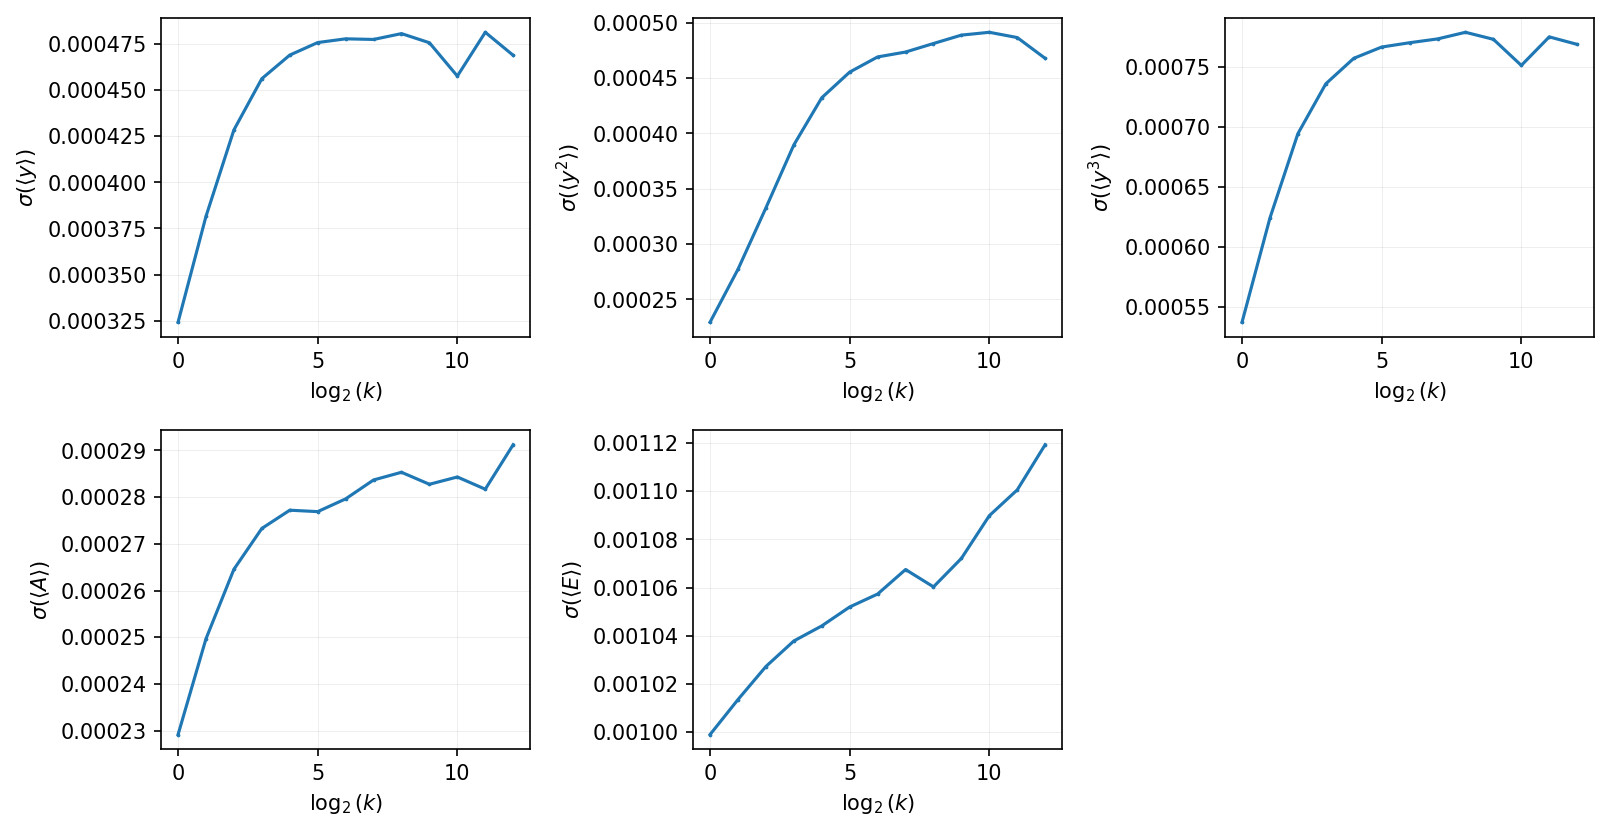
\includegraphics[width=0.8\textwidth]{../plots/bhw10_nstep1000000/nt200_therm50000/blocking_observables.png}
\caption{Andamento delle incertezze su $\langle y \rangle$, $\langle y^2 \rangle$, $\langle y^3 \rangle$, $\langle A \rangle$ e $\langle E \rangle$ in funzione dell'ampiezza dei blocchi per $\beta\hbar\omega=10$ e $N_t=200$.
L'incertezza sull'energia sembra saturare in modo peggiore. In realtà l'escursione dei valori è
relativamente piccola ma a causa dello zoom sull'asse delle ordinate appare amplificata}
\label{fig:blocking_uncertainties}
\end{figure}

\begin{figure}[H]
\centering
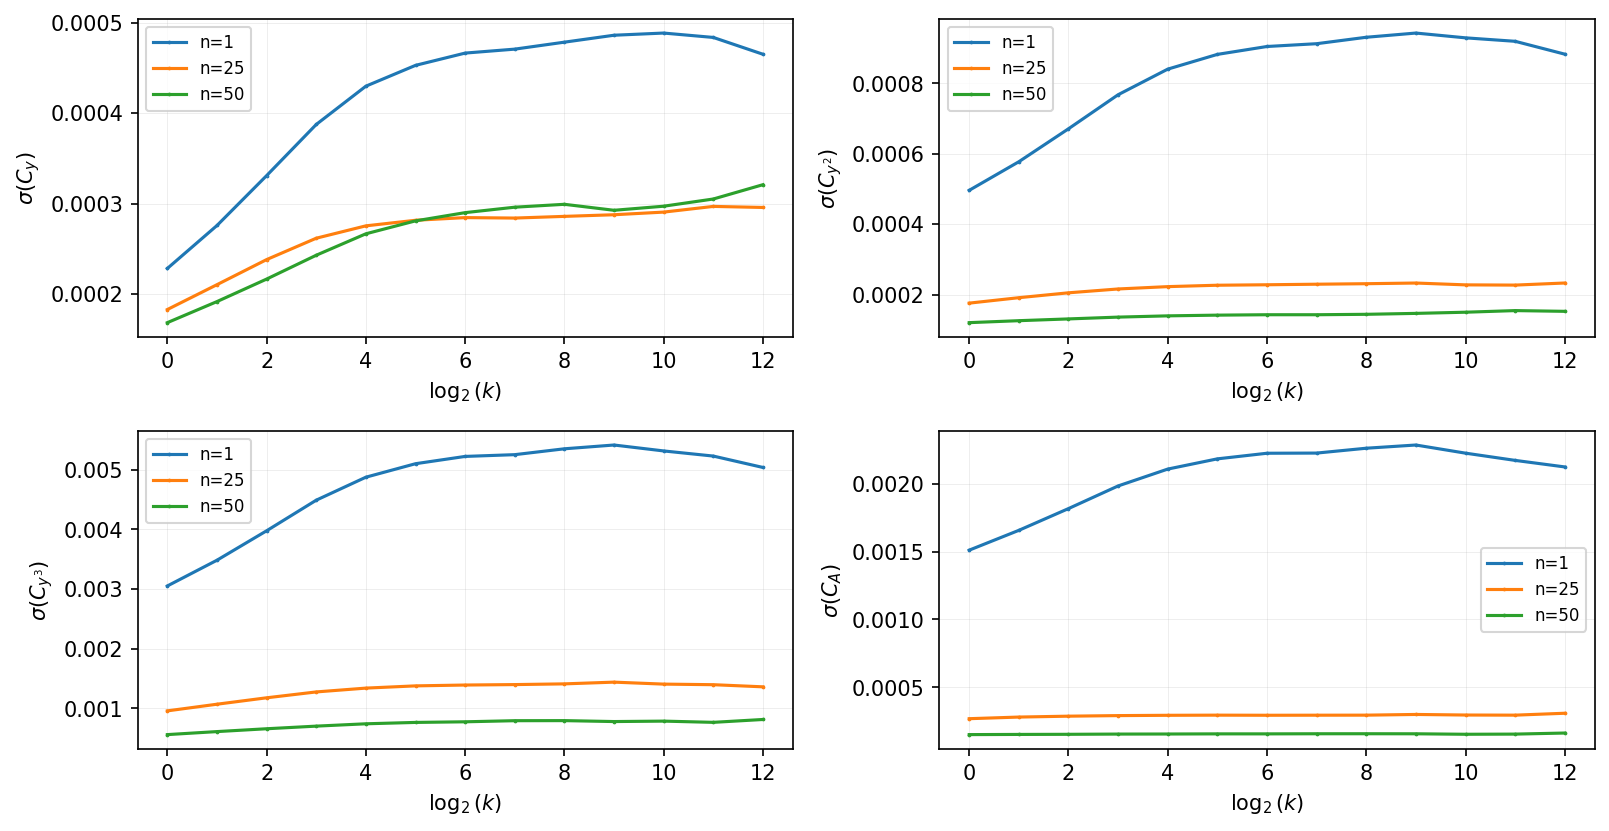
\includegraphics[width=0.8\textwidth]{../plots/bhw10_nstep1000000/nt200_therm50000/blocking_jackknife.png}
\caption{Andamento delle incertezze sui correlatori connessi per $n=1, 25, 50$ (esempio) in funzione dell'ampiezza dei blocchi per $\beta\hbar\omega=10$ e $N_t=200$}
\label{fig:jackknife_uncertainties}
\end{figure}

\subsection{Effetti di taglia finita}
Riportiamo in figura l'andamento di $\langle y \rangle$e  $\langle y^2 \rangle$
per $\beta\hbar\omega = 10$.
%Grafici con le osservabili primarie
\begin{figure}[H]
    \centering
    \begin{subfigure}[b]{0.45\textwidth}
        \centering
        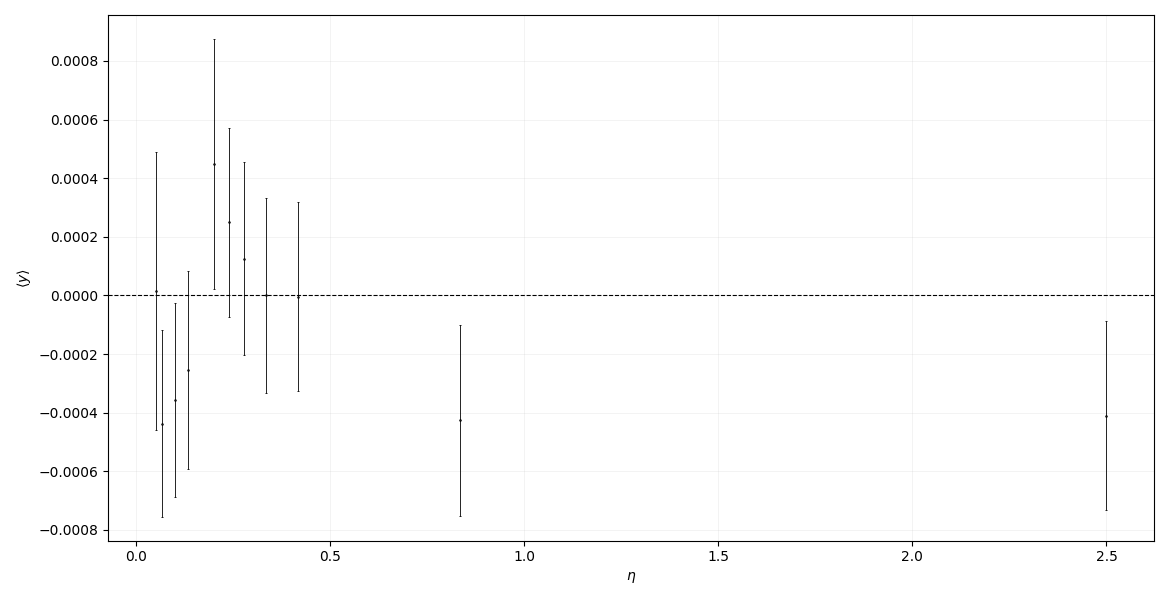
\includegraphics[width=\textwidth]{../plots/bhw10_nstep1000000/plot_y_ntherm50000.png}
        \label{subfig:grafico1}
    \end{subfigure}
    \hfill
    \begin{subfigure}[b]{0.45\textwidth}
        \centering
        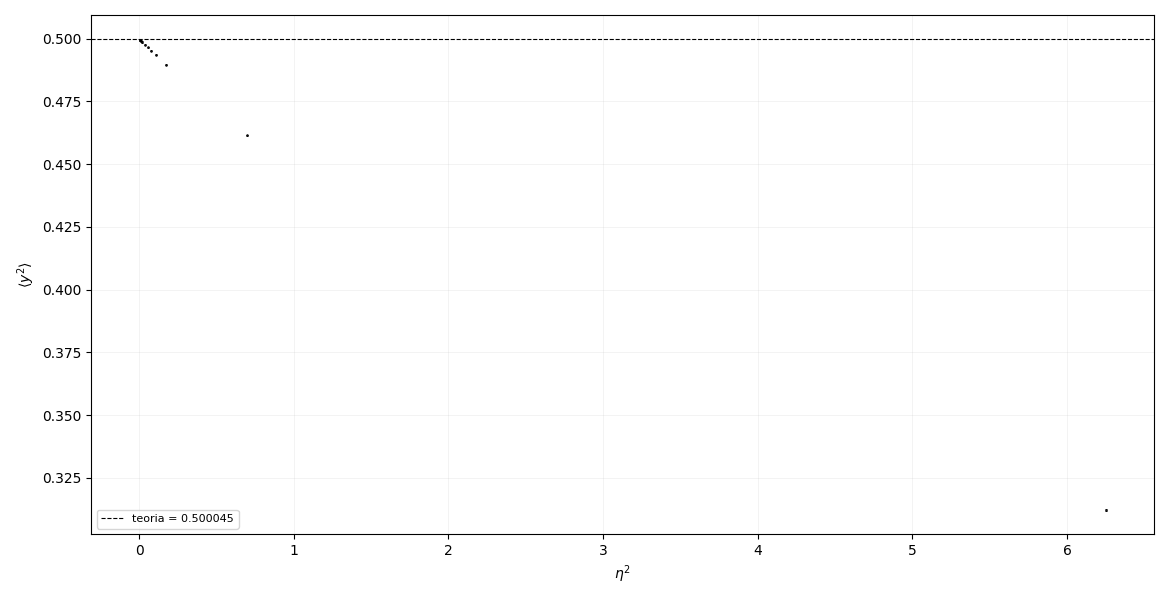
\includegraphics[width=\textwidth]{../plots/bhw10_nstep1000000/plot_y2_ntherm50000.png}
        \label{subfig:grafico2}
    \end{subfigure}
    
    \caption{Valori di $\langle y \rangle$ e $\langle y^2 \rangle$ per $\beta\hbar\omega = 10$
    in funzione di $N_t$: $y$ è compatibile con zero, mentre $y^2$ sembra compatibile col valore teorico
    di $\approx 0.5$ al limite del continuo.}
    \label{fig:combinata}
\end{figure}
Adesso mostriamo il grafico dell'energia. Si è effettuato un fit lineare in $\eta^2$
considerando i valori di $\eta < 0.5$, per testare la correttezza dell'approccio
al limite del continuo e catturare gli scostamenti $O(\eta^2)$ per effetti di finite size
(sono visibili anche gli scostamenti di ordine superiore per i valori di $\eta$ più grandi,
non inclusi nel fit).

\begin{figure}[H]
\centering
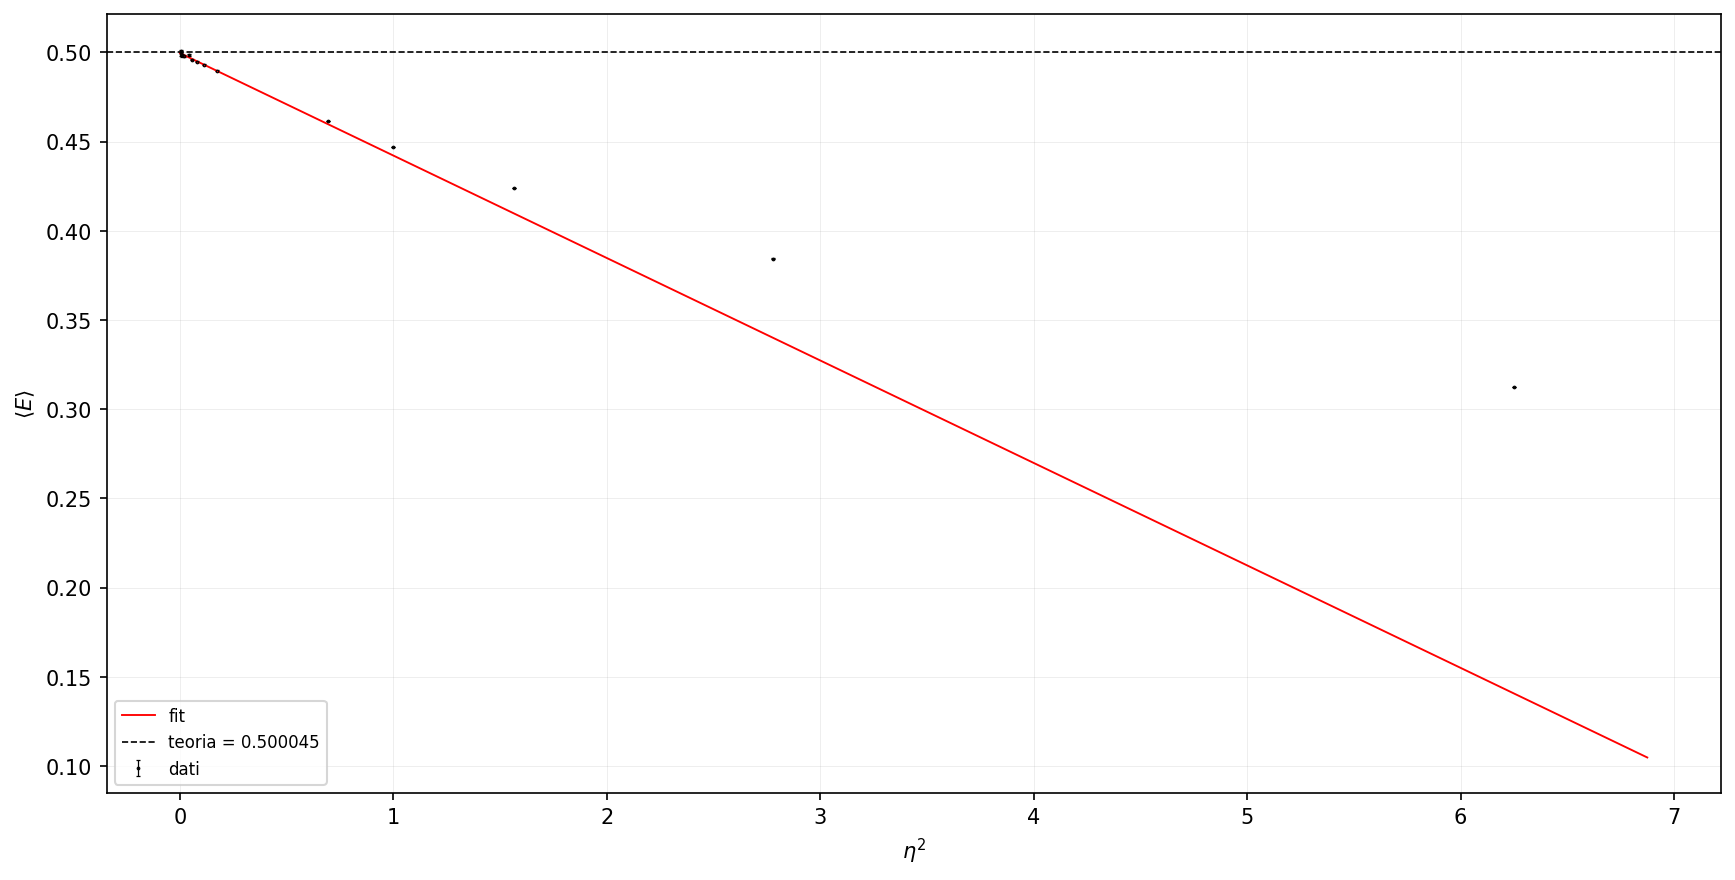
\includegraphics[width=0.8\textwidth]{../results/bhw10_nstep1000000/fits/continuum_E_20260210_125528.png}
\caption{Andamento dell'energia in funzione di $\eta^2$ per $\beta\hbar\omega=10$ e fit lineare per
i valori di $\eta < 0.5$. Sono visibili gli scostamenti di ordine superiore per i valori
più grandi di $\eta$, non inclusi nel fit.}
\label{fig:energy_continuum_fit}
\end{figure}

\begin{figure}[H]
\centering
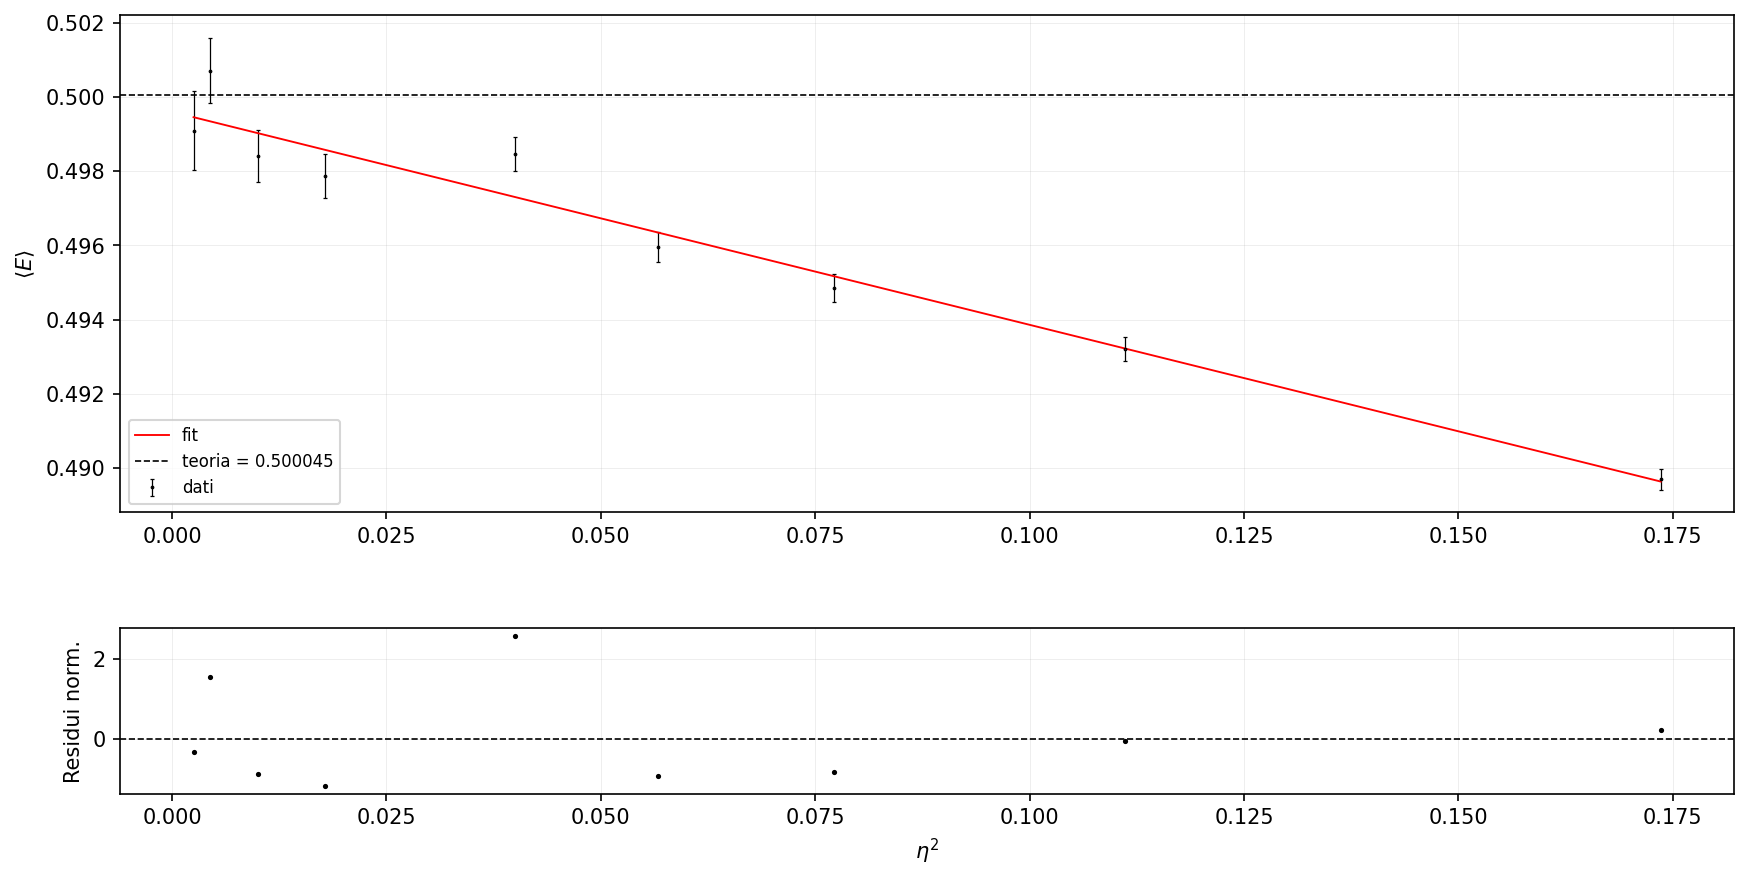
\includegraphics[width=0.8\textwidth]{../results/bhw10_nstep1000000/fits/continuum_E_20260210_125533.png}
\caption{Stesso fit dell'energia ma mostrato con i residui normalizzati, nel solo range di valori
di $\eta$ considerati per il fit. Il valore di energia al limite del continuo è compatibile con il valore teorico di
$\approx0.5$, come si vede dalla tabella riassuntiva.}
\label{fig:energy_continuum_fit_residuals}
\end{figure}

% Tabella con i risultati del fit del limite del continuo
\setlength{\heavyrulewidth}{\lightrulewidth}
\begin{table}[ht]
\centering
\caption{Risultati del fit lineare a due parametri dell'energia in funzione di $\eta^2$.
Il valore del $\chi^2$ ridotto è un po' alto, il che potrebbe essere dovuto a un caso
per statistica insufficiente o alla presenza di scostamenti non trascurabili di ordine superiore
a $\eta^2$ anche per i valori più grandi di $\eta$ considerati nel fit. Il valore di $a$ è
compatibile con il valore teorico di 0.5.}
\label{tab:risultati_fit}
\begin{tabular}{l S[table-format=1.4(3)]}
\toprule
$a$            & 0.4996(3) \\
$b$            & -0.0574(25) \\
\midrule
$\chi^2_{\nu}$ & 1.864     \\
ndf            & 7         \\
$corr(a,b)$     & -0.85 \\
\bottomrule
\end{tabular}
\end{table}

\subsection{Energia in funzione della temperatura}
Riportiamo in figura \ref{fig:energy_vs_temp} l'andamento dell'energia in funzione della temperatura.
\begin{figure}[H]
\centering
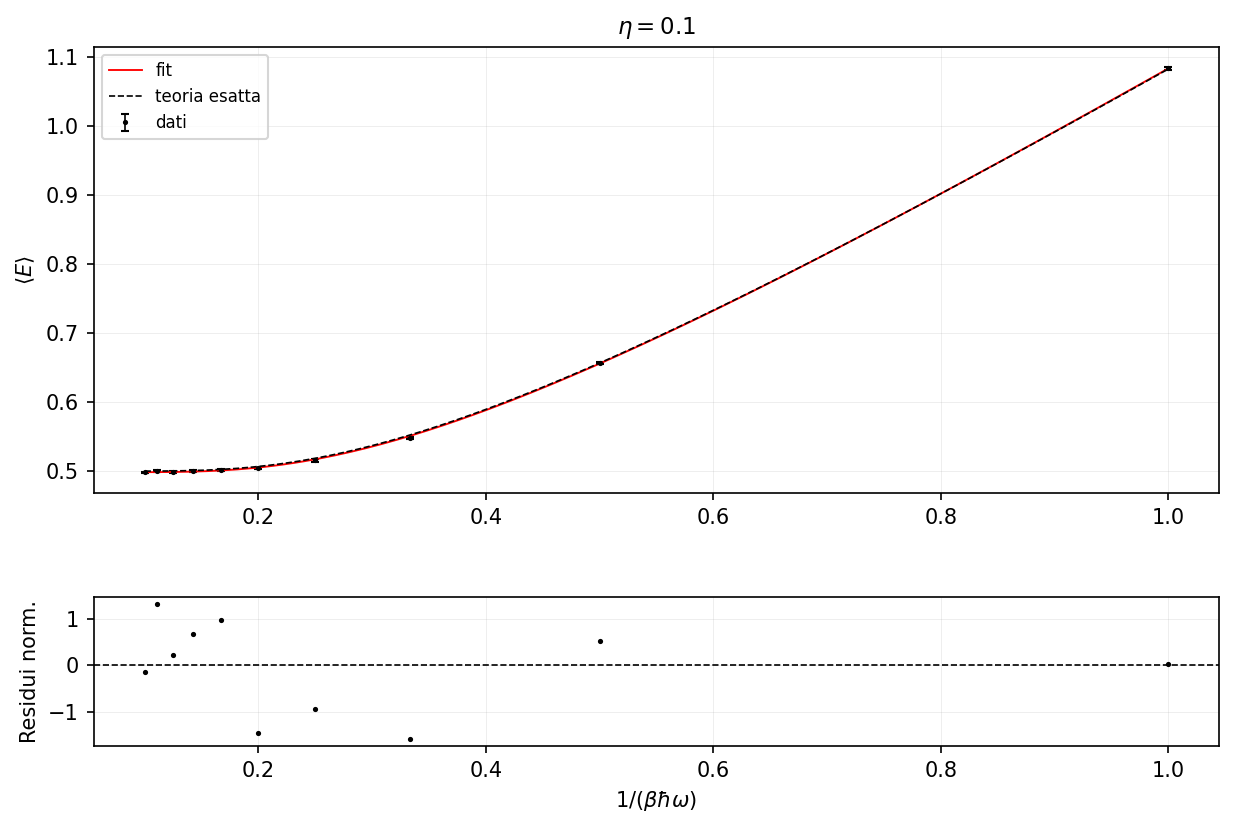
\includegraphics[width=0.8\textwidth]{../results/energy_vs_temp/fits/E_vs_T_eta0.1_20260209_182438.png}
\caption{Andamento dell'energia in funzione della temperatura per $\eta=0.1$}
\label{fig:energy_vs_temp}
\end{figure}
Abbiamo eseguito un fit a 2 parametri con modello:
\begin{equation}
    a + \frac{b}{e^{\beta\hbar\omega} - 1}
\end{equation}
% Tabella con i risultati del fit
\setlength{\heavyrulewidth}{\lightrulewidth}
\begin{table}[ht]
\centering
\caption{Risultati del fit.}
\label{tab:risultati_fit}
\begin{tabular}{l S[table-format=1.4(3)]}
\toprule
$a$            & 0.4985(4) \\
$b$            & 1.004(4) \\
\midrule
$\chi^2_{\nu}$ & 1.144     \\
ndf            & 8         \\
$corr(a,b)$     & -0.272 \\
\bottomrule
\end{tabular}
\end{table}

I valori di aspettazione di $y$, $y^3$ e $A$ sono tutti nulli per simmetria.
Il valore di aspettazione dell'energia e di $y^2$ in unità adimensionali sono uguali,
e risultano:
\begin{equation}
    \langle H \rangle = \langle y^2 \rangle = \frac{1}{2} \frac{1 + e^{-\beta\hbar\omega}}{1 - e^{-\beta\hbar\omega}}
\end{equation}

\subsection{Gap energetici}
Per estrarre i gap energetici si ricorre al gap efficace, nel caso adimensionale definito da:
\begin{equation}
    \Delta E(n) = \frac{1}{\eta} \log\left[\frac{C(n)}{C(n+1)}\right]
\end{equation}
Infatti per grandi valori di $\tau$ il correlatore connesso va come:
\begin{equation}
    C(n) \sim e^{-\tau \Delta E }
\end{equation}
Il $\Delta E$ estratto si riferisce al primo livello eccitato $E_{\overline{m}}$
tale che:
\begin{equation}
    \bra{0} O \ket{\overline{m}} \neq 0
\end{equation}
Usando la definizione di sopra otterremo una sequenza di stime del gap energetico
in funzione di $n$, che dovrebbe appiattirsi attorno a un plateau il quale corrisponde al gap.

\begin{itemize}
    \item \textbf{Gap $E_1 - E_0$}: Per stimare il primo gap energetico possiamo utilizzare
    sia il correlatore connesso di $y$ che quello di $y^3$, ma il primo risulta più accurato,
    in quanto verifica anche:
\begin{equation}
    \langle 0 | y | n \rangle = \frac{1}{\sqrt{2}} \delta_{n,1}
\end{equation}
mentre $y^3$ ha sovrapposizione non nulla anche con $0$ e $3$, quindi il profilo dei gap
converge lentamente al plateau, e prima che esso venga raggiunto in modo stabile,
i dati diventano molto rumorosi (poiché il correlatore raggiunge valori molto piccoli
e il rapporto diventa instabile, con incertezze enormi).
    \item \textbf{Gap $E_2 - E_0$}: Per stimare il secondo gap energetico si usa il correlatore
    connesso di $y^2$, che ha una sovrapposizione non nulla solo con $0$ e $2$ (quindi risulta
    particolarmente adeguato come operatore interpolante per questo gap).
    \item \textbf{Gap $E_3 - E_0$}: Per stimare il terzo gap energetico si usa il
    correlatore connesso di $A$, ma a priori questo è fattibile solo
    per l'oscillatore armonico dato che ne conosciamo la soluzione analitica. 
    Infatti $A$ è costruito ad hoc per essere proporzionale al polinomio di Hermite $H_3$,
    che sappiamo essere l'autofunzione del terzo stato eccitato. Non è possibili invece
    utilizzare $y^3$ come operatore interpolante per il terzo gap,
    poiché ha sovrapposizione non nulla anche con $1$

\end{itemize}

\begin{figure}[H]
\centering
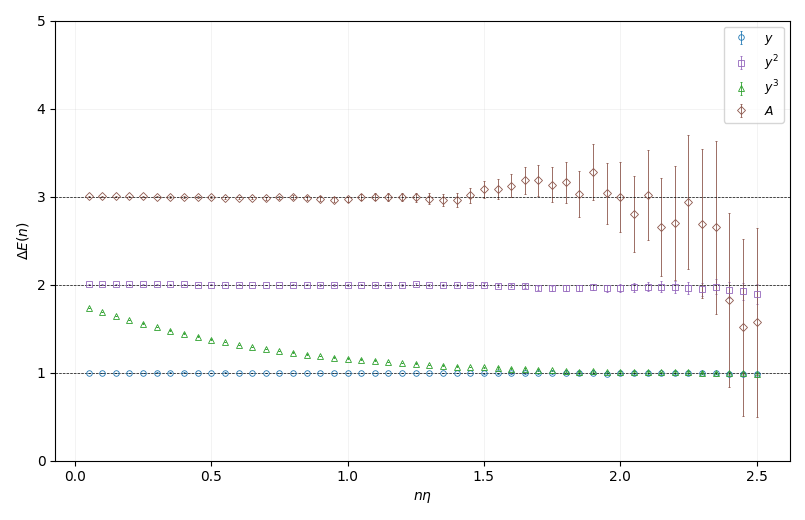
\includegraphics[width=0.8\textwidth]{../plots/bhw10_nstep1000000/nt200_therm50000/energy_gaps_n50_plot.png}
\caption{Gap efficaci con chiara manifestazione del plateau agli intervalli corretti.
Dati corrispondenti a $\beta\hbar\omega=10$ e $N_t=200$
tagliando i valori $n \eta > 2.5$, ovvero eliminando la parte maggiormente
rumorosa e affetta da incertezze più grandi (comunque nella regione mantenuta,
sono chiaramente visibili i plateau). Nella parte finale dei gap relativi a
$A$ si inizia a vedere una forte instabilità dei dati.}
\label{fig:energy_vs_temp}
\end{figure}

Possiamo effettuare un fit costante 'naive' sui dati del plateau, per estrarre i valori dei gap
energetici, tenendo a mente che i dati sono correlati tra loro, quindi è stato eseguito solo a scopo
illustrativo e non è affidabile per estrarre stime precise con le opportune incertezze.
Di seguito i risultati ottenuti:

\setlength{\heavyrulewidth}{\lightrulewidth}
\begin{table}[ht]
\centering
\caption{Fit costante sui dati del plateau, effettuato fino a $n \eta = 2.5$.}
\label{tab:gap_energetici}
\begin{tabular}{l S[table-format=1.4(3)] r}
\toprule
Gap Energetico & Stima & Valore Teorico \\
\midrule
$E_1 - E_0$ & 0.9999(3) & 1.000 \\
$E_2 - E_0$ & 2.0005(8) & 2.000 \\
$E_3 - E_0$ & 2.999(2) & 3.000 \\
\bottomrule
\end{tabular}
\end{table}

Con i risultati ottenuti, nota la soluzione analitica dell'oscillatore e la sua termodinamica,
possiamo certamente concludere che la catena di Markov implementata, campioni correttamente
la distribuzione di probabilità dei cammini, dato che le stime delle osservabili primarie e dei
gap energetici sono compatibili con i valori teorici attesi.
Aumentando la statistica si potrebbero certamente ottenere risultati più precisi al limite del continuo.

\end{document}